%%%%%%%%%%%%%%%%%%%%%%%%%%%%%%%%%%%%%%%%%

% Programming/Coding Assignment

% LaTeX Template

%

% This template has been downloaded from:

% http://www.latextemplates.com

%

% Original author:

% Ted Pavlic (http://www.tedpavlic.com)

%

% Note:

% The \lipsum[#] commands throughout this template generate dummy text

% to fill the template out. These commands should all be removed when 

% writing assignment content.

%

% This template uses a Perl script as an example snippet of code, most other

% languages are also usable. Configure them in the "CODE INCLUSION 

% CONFIGURATION" section.

%

%%%%%%%%%%%%%%%%%%%%%%%%%%%%%%%%%%%%%%%%%



%----------------------------------------------------------------------------------------

%	PACKAGES AND OTHER DOCUMENT CONFIGURATIONS

%----------------------------------------------------------------------------------------



\documentclass{article}



\usepackage{fancyhdr} % Required for custom headers

\usepackage{lastpage} % Required to determine the last page for the footer

\usepackage{extramarks} % Required for headers and footers

\usepackage[usenames,dvipsnames]{color} % Required for custom colors

\usepackage{graphicx} % Required to insert images

\usepackage{listings} % Required for insertion of code

\usepackage{courier} % Required for the courier font

\usepackage{textcomp} % Required for the courier font

\usepackage{float} % for positioning pictures

\usepackage{lipsum} % Used for inserting dummy 'Lorem ipsum' text into the template



% Margins

\topmargin=-0.45in

\evensidemargin=0in

\oddsidemargin=0in

\textwidth=6.5in

\textheight=9.0in

\headsep=0.25in



\linespread{1.1} % Line spacing



% Set up the header and footer

\pagestyle{fancy}

\chead{\hmwkClass\ (\hmwkClassInstructor\ \hmwkClassTime): \hmwkTitle} % Top center head

\rhead{\firstxmark} % Top right header

\lfoot{\lastxmark} % Bottom left footer

\cfoot{} % Bottom center footer

\rfoot{Page\ \thepage\ of\ \protect\pageref{LastPage}} % Bottom right footer

\renewcommand\headrulewidth{0.4pt} % Size of the header rule

\renewcommand\footrulewidth{0.4pt} % Size of the footer rule



\setlength\parindent{0pt} % Removes all indentation from paragraphs



%----------------------------------------------------------------------------------------

%	CODE INCLUSION CONFIGURATION

%----------------------------------------------------------------------------------------



% Creates a new command to include a perl script, the first parameter is the filename of the script (without .pl), the second parameter is the caption

\newcommand{\Javas}[2]{

\begin{itemize}

\item[]\lstinputlisting[caption=#2,label=#1]{#1.java}

\end{itemize}

}



\definecolor{MyDarkGreen}{rgb}{0.0,0.4,0.0} % This is the color used for comments





%----------------------------------------------------------------------------------------

%	NAME AND CLASS SECTION

%----------------------------------------------------------------------------------------



\newcommand{\hmwkTitle}{Programming Assignment\ \#3} % Assignment title

\newcommand{\hmwkDueDate}{Friday,\ November\ 07,\ 2014} % Due date

\newcommand{\hmwkClass}{CS553\ } % Course/class

\newcommand{\hmwkClassTime}{} % Class/lecture time

\newcommand{\hmwkClassInstructor}{Ioan Raicu} % Teacher/lecturer

\newcommand{\hmwkAuthorName}{Thomas Dubucq / Tony Forlini / Virgile Landeiro} % Your name



%----------------------------------------------------------------------------------------

%	TITLE PAGE

%----------------------------------------------------------------------------------------



\title{
\vspace{2in}
\textmd{\textbf{\hmwkClass:\ \hmwkTitle}}\\
\normalsize\vspace{0.1in}\small{Due\ on\ \hmwkDueDate}\\
\vspace{0.1in}\large{\textit{\hmwkClassInstructor\ \hmwkClassTime}}
\vspace{3in}
}



\author{\textbf{\hmwkAuthorName}}
\date{} % Insert date here if you want it to appear below your name



%----------------------------------------------------------------------------------------



\begin{document}



\maketitle



%----------------------------------------------------------------------------------------

%	TABLE OF CONTENTS

%----------------------------------------------------------------------------------------



%\setcounter{tocdepth}{1} % Uncomment this line if you don't want subsections listed in the ToC



\newpage

\tableofcontents

\newpage



%----------------------------------------------------------------------------------------

%	Introduction

%----------------------------------------------------------------------------------------



% To have just one problem per page, simply put a \clearpage after each problem



\section{Introduction}

The goal of this programming assignment is to enable us to gain experience programming with:

\begin{itemize}

  \item Google App Engine (https://appengine.google.com/)

  \item Google Cloud Storage (https://cloud.google.com/storage/)

  \item Google's Memcache (https://cloud.google.com/appengine/docs/adminconsole/memcache)\\

\end{itemize}

This assignment topic is to discover Google App Engine (GAE) programming. Specifically, this assignment deals with Google Cloud Storage (GCS) and Google Memcache. The goal of this assignment is to create a distributed storage system using the 3 aforementioned Google services. This storage system should have a different behaviour depending on the size of the file to upload, to improve the responsiveness of the whole system.



Google App Engine is a Platform as a Service (PaaS), released in September 2011. GAE allows developpers to implement their applications in several different languages : Python, Java, PHP and Go. GAE apps need to use a web page interface and can be scaled automatically. With GAE comes a lot of different features such as Google Memcache that we will use in this assignment, but also storing, images handling, MapReduce and other features.



Google Cloud Storage is an Infrastructure as a Service (IaaS), made available in March 2010. It allows users to store data on Google's Cloud. Security and redundancy are handled by the cloud's apis, and this service can be accessed by other Google products. In this assignment, we will access it via Google App Engine.



Google Memcache is a GAE feature that allows users to store data of relatively small size on cached memory, which allows faster writing/reading than the GCS. Memcache is separated in 2 classes : dedicated and shared. Dedicated memcache is exclusively allocated to one's application, but has a billing price. On the other end shared memcache is split among all GAE apps and use a best-effort policy to provide space to them. In this assignment we will use the later.



\section{Implementation}

We decided to implement this assignement in Python.



The developement of a GAE application in Python requires, among others, both cloudstorage and google-cloud-sdk apis, both provided by Google.



The difficulty of this project is that the code is a server-based one, so data retrieving from the client has to be done via HTML requests. Unfortunately HTML requests cannot exceed 32MB. The whole system is subdivided in a front end and back end part. These two parts' implementation is detailed in the following sections.

 

\subsection{Front end}

The front end code is the actual interface with the user. It consists in a HTML page where the user can specify its requests to the storage system. 

The front end  interface has basically two main purposes, retrieving users' requests and sending them to the GAE app. The are fulfilled with two functions get and post, that respectively retrieve instructions from the user, and send them to the GAE app.

The functions get and post rely on the cgi library that allows the handling and processing of HTML forms.





The htlm forms are linked to a particular URL in which the POST values are retrieved, then treated in a corresponding class with the StorageApi methods and finally displayed using the GET method. We defined one URL per implemented function from the StorageApi. We will explain the implementation of the StorageApi methods in a further section. We used different kind of inputs in our forms to retrieve the file names or content as well as buttons.



We implemented a first version which doesn't handle the upload of big files, then we used blobstore to solve this problem even if the instructions were to not use blobstore since we only use it as a third party.

To retrieve a file from the user filesystem to the web application, we used a blobstore file upload input as a third party since we are unable to retrieve files bigger than 32MB from a simple file input within the html form. 





Another level of indirection is added with the use of blobstore to retrieve big files because blobstore uses a "blobkey" and a "userkey" to directly put the file content within google cloud storage. The first key points on the file name while the second points to the file content. Thus a dictionnary is created by blobstore while inserting a file in google cloud storage to list the different keys. Consequently we have to make the correspondance between the filename from the user filesystem and the "userkey" from the blobstore dictionnary.



Eventually the web page consist in a list of the API's methods to insert, check remove a file or obtain information about the state of the storage (both cache and google cloud storage). After submitting a form, the user is redirected on another page with the URL coresponding with the method used from the API. Sessions are used to keep the blobstore key dictionnary actualised so that we can retrieve the data already added to the storage. Note that one needs to refresh the main page after adding a file to the storage in order to be able to retrieve the files afterwards.

The web interface is accessible in the following link: http://cs553-cloudcomputing-prog3.appspot.com



\subsection{Back end}

The back end code is the one running on Google App Engine servers. Its role is to treat the files send by the users and store them. It is also responsible for retrieving data from the storage system, and manage files deletions.





We implemented the following functions to interact with our storage system:



\begin{itemize}

	\item insert(key, blobinfo) : 

	adds the file located at "value" using "key" as a name to the whole storage system. If the file is small enough (\textless100 kB), it is added to memcache. The file is always added to GCS whatever its size. We use the blobstore to handle the upload of files of more than 32MB. Then the files are added to both the memcache and gcs id the files is less or equal than 100KB and only gcs when the file is more than 100KB. Before actually adding the file, the content is retrieved from the blobstore and then added to gcs or memcache. We delete the content of the file on blobstore right after we add it to the regular storage.

	\item check(key) : 

	verifies if a file named key exists in the whole storage system using the check\_cache() and the check\_storage() functions.

	\item find(key) :

	Retrieves the contents of a file named key as a string from the cache or the distributed storage system by reading in the gcs file corresponding to the right blobkey found in the dictionnary.

	\item remove(key) :

	deletes the file named key from the cache and the distributed storage system using the delete() functions from memcache and gcs APIs bound with the corresponding blobkey.

	\item listing(string=None) :

	retrives a list of all file names stored as an array. It is possible to specify a regex to this function to only get the matching file subset using the gcs listbucket() function.

	\item check\_storage(key) :

	checks if a file named key exists in the GCS bucket by checking that the key appears in the return value of the listing() function.

	\item check\_cache(key) :

	checks if a file named key exists in memcache using the memcache get() method with the corresponding key. 

	\item remove\_all\_cache() :

	removes all files from the cache using the memcache flush\_all() method.

	\item remove\_all() :

	removes all files from the whole storage system (GCS \& memcache) using the remove\_all\_cache() method and by using the gcd delete() method on all the files of a bucket found in listbucket().

	\item cache\_size\_mb() :

	returns the space allocated to the files in memcache (in MB) using the get\_stats() method with the "bytes" attribute.

	\item cache\_size\_elem() :

	returns the total number of files in memcache using the get\_stats() method with the "items" attribute.

	\item storage\_size\_mb() :

	returns the total space allocated to files in GCS by summing on the size of each file in the bucket found in file.st\_size

	\item storage\_size\_elem() :

	returns the total number of files stored in GCS by summing on the number of items in listbucket().

	\item find\_in\_file(key,string) :

	searches for a regex in the file named key using the search() method.

	\item listing\_regex(key,string) :

	retrieves the file names matching the regex string as an array using a filter on every files content that matches the string and returning the corresponding key.\\

\end{itemize}



\section{Performance}

The performance evaluation of our implementation consists in testing 3 different types of request : upload, access and deletion of a dataset. These request will be answered using 1 or 4 threads, and with and without the memcache feature.



\subsection{Dataset}

The dataset used for this performance testing includes 411 files for a total size of 311MB. These files are distributed as following

\begin{itemize}

\item 100 files of 1KB

\item 100 files of 10KB

\item 100 files of 100KB

\item 100 files of 1MB

\item 10 files of 10MB

\item 1 files of 100MB\\

\end{itemize}

These files are generated with a python script that is part of the code submission for this assignement. They have random alpha-numerical 10-characters-long names and consist in 100 bytes random string lines.



\subsection{Benchmark}

There is a total of 12 experiements to conduct. The testing will measure the average throughput in MB/s for the upload and access phases, and the latency for the 3 phases. We implemented two version of the application, the first one doesn't handle the upload of files of more than 32MB, and the second one handles it by using blobstore. Nevertheless, we were unable to measure the transmission time for an upload using the blobstorage. Thus we only computed the benchmark on a version which doesn't hanlde upload of big files.

\begin{figure}[!ht]
\centering
\begin{tabular}{cc}
\includegraphics[width=15cm, height=9cm]{Latency}
\end{tabular}
\caption{Average Latency for 115 MB}
\end{figure}

\begin{figure}[!ht]
\centering
\begin{tabular}{cc}
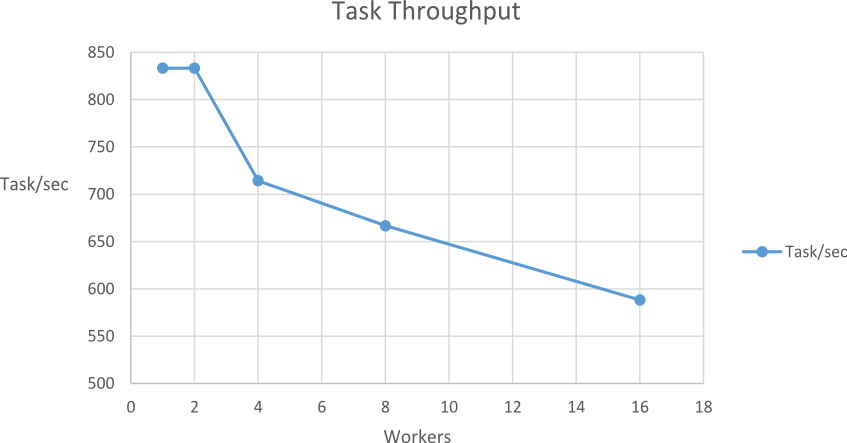
\includegraphics[width=15cm, height=9cm]{Throughput}
\end{tabular}
\caption{Throughput for 115 MB}
\end{figure}

\subsection{Results}
We were unable to mesure the benchmark on the whole dataset, because the http requests were longer than 60 seconds for 311MB which caused deadline exceeded errors. Thus we only uploaded 115 MB and we measured the Insert function and the delete function since the find function since the memory available on the GAE instance wasn't big enough to handle such intensive memory usage. We both measured the latency and throughput with the benchmark code and the web browser tools in order to get objective results and to make sure that our results were in a right range of values. We found that the operations are slower when using both memcache and gcs which makes sense because there is an overhead involved in removing extra files from memcache. Our results with the benchmark are slightly the different as the web browser tools because the latency to access the GAE insance is added with the web browser latency computation. 
\subsection{Comparison to Amazon S3}



In this section we will study the pricing details of high workload applications assuming that our dataset is now of 411 million files, that stores 311 TB. The 1 Million users need to transfer 311 TB of data to the cloud, and then read 622 TB of data from the cloud.We assume that the workload is uniformly spread out over one month. We first study the Amazon S3 case using the Amazon Web Services Simple Monthly Calculator: http://calculator.s3.amazonaws.com/calc5.html\\





\begin{center}

   \begin{tabular}{ | c | c | }

     \hline

     Amazon S3 &  \\ \hline

     Storage & 311 TB \\ \hline

     PUT/COPY/POST/LIST Requests & 1000000 \\ \hline

     GET and Other Requests & 1000000\\ \hline

     Data Transfer Out & 622 TB \\ \hline

     Data Transfer In & 311 TB\\ \hline

     Total & 110,607\$ \\

     \hline

   \end{tabular}

 \end{center}

 

Now let's take a look at the GAE pricing fo our high workload application. We gathered the pricing informations from google app engine pricing page:  https://cloud.google.com/appengine/pricing\\



\begin{center}

   \begin{tabular}{ | c | c | }

	\hline

    GAE Pricing & \\ \hline

	Instances 	(Instance hours) &	\$0.05\\ \hline

	Outgoing Network Traffic (Gigabytes) &	\$0.12\\ \hline

	Incoming Network Traffic 	(Gigabytes) &	Free\\ \hline

	Datastore Storage 	(Gigabytes per month) &	\$0.18\\ \hline

	Blobstore, Logs, and Task Queue Stored Data 	(Gigabytes per month) &	\$0.026\\ \hline

	Dedicated Memcache 	(Gigabytes per hour) &	\$0.06\\ \hline

	Logs API 	(Gigabytes) &	\$0.12\\ \hline	

	SSL Virtual IPs(Virtual IP per month) &	\$39.00\\

	\hline

   \end{tabular}

 \end{center}



We compute the estimated price on the basis of the use of data transfer and the use of the memcache and google cloud storage according to the size of the file. Here is the estimates total price for our application:



\begin{center}

   \begin{tabular}{ | c | c | }

     \hline

     Google App Engine &  \\ \hline

     DataStore 300 TB  & 55,296 \$\\ \hline

     Memcache 11TB  & 675 \$ \$\\ \hline

     Data Transfer Out 622 TB & 76,431 \$ \\ \hline

     Data Transfer In 311 TB & FREE\\ \hline

     Total & 132,438\$ \\

     \hline

   \end{tabular}

 \end{center}

 



Finally we observe that the overall price for Google App Engine is more expensive than the price of deploying the application on Amazon Web Services.

First the fact that one needs to setup the whole architecture on AWS in order to deploy an application explains the lower cost. Second, high workload and high throughput application are usually better designed using AWS rather than GAE which is more startup application oriented. The higher workload, the lower the monthly price per unit on AWS, besides the pricing is fixed on GAE which prevent from making savings with heavy workloads.  



%----------------------------------------------------------------------------------------

\newpage



\title{\vspace{2in}
\LARGE
\textmd{\textbf{Sources}\\
}
\normalsize
\\
Google App Engine (https://appengine.google.com/\\
Google Cloud Storage (https://cloud.google.com/storage/)\\
Google's Memcache (https://cloud.google.com/appengine/docs/adminconsole/memcache)\\
Google app engine pricing page: https://cloud.google.com/appengine/pricing\\
Amazon Web Services Simple Monthly Calculator: http://calculator.s3.amazonaws.com/calc5.html\\
http://www.vogella.de/articles/GoogleAppEngineJava/article.html\\ http://www.ibm.com/developerworks/java/library/j-gaej1/\\
\end{document}

